\documentclass[notes,11pt, aspectratio=169, xcolor=table]{beamer}

\usepackage{pgfpages}
% These slides also contain speaker notes. You can print just the slides,
% just the notes, or both, depending on the setting below. Comment out the want
% you want.
\setbeameroption{hide notes} % Only slide
%\setbeameroption{show only notes} % Only notes
%\setbeameroption{show notes on second screen=right} % Both

\usepackage{helvet}
\usepackage[default]{lato}
\usepackage{array}
\usepackage[utf8]{inputenc} 

\newtheorem{proposition}{Proposition}

\usepackage{tikz}
\usetikzlibrary{shapes.geometric}
\usepackage{pgfplots}
\usepackage{graphicx}
\usepackage{verbatim}
\setbeamertemplate{note page}{\pagecolor{yellow!5}\insertnote}
\usetikzlibrary{positioning}
\usetikzlibrary{snakes}
\usetikzlibrary{calc}
\usetikzlibrary{arrows}
\usetikzlibrary{decorations.markings}
\usetikzlibrary{shapes.misc}
\usetikzlibrary{matrix,shapes,arrows,fit,tikzmark}
\usepackage{amsmath}
\usepackage{mathpazo}
\usepackage{hyperref}
\usepackage{lipsum}
\usepackage{multimedia}
\usepackage{graphicx}
\usepackage{multirow}
\usepackage{graphicx}
\usepackage{dcolumn}
\usepackage{bbm}
\usepackage[style=authoryear,sorting=nyt,uniquename=false]{biblatex}
\newcommand{\blue}[1]{\textcolor{blue}{#1}}
\newcommand{\white}[1]{\textcolor{white}{#1}}

\addbibresource{references.bib} 

\newcolumntype{d}[0]{D{.}{.}{5}}

\def\@@mybluebox[#1][#2]#3{
    \sbox\mytempbox{#3}%
    \mytemplen\ht\mytempbox
    \advance\mytemplen #1\relax
    \ht\mytempbox\mytemplen
    \mytemplen\dp\mytempbox
    \advance\mytemplen #2\relax
    \dp\mytempbox\mytemplen
    \colorbox{myblue}{\hspace{1em}\usebox{\mytempbox}\hspace{1em}}}


\usepackage{changepage}
\usepackage{appendixnumberbeamer}
\newcommand{\beginbackup}{
   \newcounter{framenumbervorappendix}
   \setcounter{framenumbervorappendix}{\value{framenumber}}
   \setbeamertemplate{footline}
   {
     \leavevmode%
     \hline
     box{%
       \begin{beamercolorbox}[wd=\paperwidth,ht=2.25ex,dp=1ex,right]{footlinecolor}%
%         \insertframenumber  \hspace*{2ex} 
       \end{beamercolorbox}}%
     \vskip0pt%
   }
 }
\newcommand{\backupend}{
   \addtocounter{framenumbervorappendix}{-\value{framenumber}}
   \addtocounter{framenumber}{\value{framenumbervorappendix}} 
}


\usepackage{graphicx}
\usepackage[space]{grffile}
\usepackage{booktabs}

% These are my colors -- there are many like them, but these ones are mine.
\definecolor{blue}{RGB}{0,114,178}
\definecolor{red}{RGB}{213,94,0}
\definecolor{yellow}{RGB}{240,228,66}
\definecolor{green}{RGB}{0,158,115}

\hypersetup{
  colorlinks=false,
  linkbordercolor = {white},
  linkcolor = {blue}
}


%% I use a beige off white for my background
\definecolor{MyBackground}{RGB}{255,253,218}

%% Uncomment this if you want to change the background color to something else
%\setbeamercolor{background canvas}{bg=MyBackground}

%% Change the bg color to adjust your transition slide background color!
\newenvironment{transitionframe}{
  \setbeamercolor{background canvas}{bg=yellow}
  \begin{frame}}{
    \end{frame}
}

\setbeamercolor{frametitle}{fg=blue}
\setbeamercolor{title}{fg=blue}
\setbeamertemplate{footline}[frame number]
\setbeamertemplate{navigation symbols}{} 
\setbeamertemplate{itemize items}{-}
\setbeamercolor{itemize item}{fg=blue}
\setbeamercolor{itemize subitem}{fg=blue}
\setbeamercolor{enumerate item}{fg=blue}
\setbeamercolor{enumerate subitem}{fg=blue}
\setbeamercolor{button}{bg=MyBackground,fg=blue,}



% If you like road maps, rather than having clutter at the top, have a roadmap show up at the end of each section 
% (and after your introduction)
% Uncomment this is if you want the roadmap!
% \AtBeginSection[]
% {
%    \begin{frame}
%        \frametitle{Roadmap of Talk}
%        \tableofcontents[currentsection]
%    \end{frame}
% }
\setbeamercolor{section in toc}{fg=blue}
\setbeamercolor{subsection in toc}{fg=red}
\setbeamersize{text margin left=1em,text margin right=1em} 

\newenvironment{wideitemize}{\itemize\addtolength{\itemsep}{10pt}}{\enditemize}

\usepackage{environ}
\NewEnviron{videoframe}[1]{
  \begin{frame}
    \vspace{-8pt}
    \begin{columns}[onlytextwidth, T] % align columns
      \begin{column}{.58\textwidth}
        \begin{minipage}[t][\textheight][t]
          {\dimexpr\textwidth}
          \vspace{8pt}
          \hspace{4pt} {\Large \sc \textcolor{blue}{#1}}
          \vspace{8pt}
          
          \BODY
        \end{minipage}
      \end{column}%
      \hfill%
      \begin{column}{.42\textwidth}
        \colorbox{green!20}{\begin{minipage}[t][1.2\textheight][t]
            {\dimexpr\textwidth}
            Face goes here
          \end{minipage}}
      \end{column}%
    \end{columns}
  \end{frame}
}

\title[]{International Trade: Lecture XX}
\subtitle[]{Diverse Firms and Trade: The Melitz Model}
\author[Góes]
{Carlos Góes\inst{1}}
\date{Fall 2025}
\institute[GWU]{\inst{1} George Washington University }



\begin{document}

%%% TIKZ STUFF
\tikzset{   
        every picture/.style={remember picture,baseline},
        every node/.style={anchor=base,align=center,outer sep=1.5pt},
        every path/.style={thick},
        }
\newcommand\marktopleft[1]{%
    \tikz[overlay,remember picture] 
        \node (marker-#1-a) at (-.3em,.3em) {};%
}
\newcommand\markbottomright[2]{%
    \tikz[overlay,remember picture] 
        \node (marker-#1-b) at (0em,0em) {};%
}
\tikzstyle{every picture}+=[remember picture] 
\tikzstyle{mybox} =[draw=black, very thick, rectangle, inner sep=10pt, inner ysep=20pt]
\tikzstyle{fancytitle} =[draw=black,fill=red, text=white]
%%%% END TIKZ STUFF



%----------------------------------------------------------------------%
%-------------------       TITLE PAGE       ---------------------------%
%----------------------------------------------------------------------%





%----------------------------------------------------------------------%






%----------------------------------------------------------------------%
%----------------------------------------------------------------------%

%----------------------------------------------------------------------%
\frame{\titlepage}
\addtocounter{framenumber}{-1}
%----------------------------------------------------------------------%

\section{Intro and recap}

\begin{frame}{So far...}
\begin{wideitemize}
    \item ``Standard trade model'' (or neoclassical trade model)
        \begin{itemize}
            \item constant returns to scale + perfect competition
            \item trade happens because countries are different
        \end{itemize}
    \item Intraindustry trade model (Krugman model)
    \begin{itemize}
        \item Trade happens because people have preferences over \blue{differentiated goods}
        \item Monopolistic competition
        \item Substitution across goods
    \end{itemize}
\end{wideitemize}
\end{frame}

\begin{frame}{Today: Diverse Frames and Trade}

\begin{wideitemize}
    \item In practice, nontraded varieties arise even within industries
    \item Non-exporters and exporters coexist
    \item  What explains their different trading behavior?
    \item  Firms differ in innate individual characteristics. \\
 \qquad (e.g: consumer appeal, quality, productivity)
    \item  Revisit monopolistic competition, with diversity in marginal costs
\end{wideitemize}
    
\end{frame}

\begin{frame}{Exporter Premia in U.S. Manufacturing 2002}
\begin{table}[htbp]
\centering
\label{tab:exporter-premia}
\begin{tabular}{lccc}
\toprule
& \multicolumn{3}{c}{\textbf{Comparison}} \\
\cmidrule(lr){2-4}
& any industry & same industry & same industry \\
&              &               & and given firm size \\
\midrule
Employment                 & 229\% & 164\% & 8\% \\
Sales                      & 339\% & 194\% & 8\% \\
Capital per worker         & 38\%  & 13\%  & 4\% \\
Share non-production workers & 21\%  & 12\%  & 21\% \\
Average wage               & 19\%  & 6\%   & 6\% \\
Value-added per worker     & 30\%  & 12\%  & 11\% \\
Total factor productivity  & 2\%   & 3\%   & 5\% \\
\bottomrule
\multicolumn{4}{p{0.85\linewidth}}{\footnotesize \textit{Source:} \href{https://www.aeaweb.org/articles?id=10.1257/jep.21.3.105}{Bernard, Jensen, Redding \& Schott (2007)}.}\\
\multicolumn{4}{p{0.85\linewidth}}{\footnotesize \textit{Note:} Results from OLS regressions of the log firm characteristic on an indicator variable for firm’s export status and controls (industry fixed effect and log employment).}
\end{tabular}
\end{table}
    
\end{frame}

\begin{frame}{Superior Exporter Performance}

\begin{wideitemize}
    \item  Superior exporter performance: Is it learning from exporting?
    \item Or is it the sorting of the highly competitive firms into export markets?
    \item Evidence points to sorting of most competitive firms into exporting
    \item Only highly competitive firms generate profits to cover fixed entry cost
    \item Melitz (2003): Firm dynamics and trade openness
    
\end{wideitemize}

\end{frame}


\begin{frame}{Marc Melitz (1968–)}
\begin{columns}
    \begin{column}{0.65\textwidth}
        \begin{wideitemize}
            \item Born: 1968, United States
            \item Professor at Harvard University; leading figure in modern trade theory
            \item Introduced diverse firms into international trade
            \item Research shows how only the most productive firms export and trade liberalization reallocates market shares
            \item Fellow of the Econometric Society; influential in policy and academic debates on globalization
            \item Future Nobel laureate
            \item Generous guy (answers my emails)
        \end{wideitemize}
    \end{column}
    
    \begin{column}{0.35\textwidth}
        \centering
        
\includegraphics[width=\linewidth]{figs/melitz_marc030r.jpeg} 
        \vspace{0.2cm}
        \scriptsize\textit{Marc Melitz (source: Harvard University)}
    \end{column}
\end{columns}
\end{frame}


\section{The Melitz Model}

\begin{frame}{The Melitz Model}
\begin{wideitemize}
            \item Builds on Krugman’s monopolistic competition framework
            \item Adds \blue{diverse firms}
            \item Firms will differ in their productivity and marginal cost
            \item Key new mechanism:
            \begin{itemize}
                \item only productive enough firms enter the market
                \item only most productive firms export
            \end{itemize}
            \item Trade liberalization leads to \blue{reallocation} of resources toward more productive firms
\end{wideitemize}
\end{frame}

\begin{frame}{The Krugman Model}

\begin{wideitemize}
    \item Intra-industry Trade Model: trade in goods within the same industry
    \item Trade because of \blue{differentiated goods}
    \item Firms have a monopoly of the type of good $\varphi$ they produce
    \item Upon entry, firms maximize operational profits (Stage 2).
    \item  However, free entry erodes profits to zero in equilibrium (Stage 1)
\end{wideitemize}
    
\end{frame}

\begin{frame}{The Melitz Model}
    \begin{wideitemize}
        \item \blue{Number} of factors of production: 1 (labor $\ell$, but can be generalized)\\
        \qquad \textcolor{gray}{(no specific factors)}
        
    \item<2-> \blue{Mobility} of factors of production: yes
    
    \item<3-> Number of \blue{sectors}: one 

    \item<4-> Number of \blue{goods}: (countably) many   

    \item<5-> Number of countries: 2 ($H$ and $F$)

    \item<6-> Imperfect competition, variable transport costs, fixed entry costs

    \item<6-> \blue{Key force}: differences in technologies between firms
    \end{wideitemize}    
\end{frame}

\section{Production}

\begin{frame}{Production with firm heterogeneity}

\begin{wideitemize}
    \item Producers of each good $\varphi$ have a monopoly over the production of their good
    \item They also will have to pay a fixed cost $\bar{f}$ to set up shop (only if they enter the market)

    \item To produce a given quantity $q_i(\varphi)$, labor used is:

    \begin{equation*}
         \ell = \bar{f} + a(\varphi)q_i(\varphi) \iff q_i(\varphi) = \frac{1}{a(\varphi)} (\ell - \bar{f})
    \end{equation*}

    \item $a(\varphi)$: denotes how many workers are necessary to produce a single unit of good $\varphi$. \\
    \qquad (\blue{unit labor requirements} -- up to here, same as Krugman) 

    \item<2-> Assume that $a(\varphi)$ is \textbf{decreasing} in the order of the good $\varphi$. Specifically, we will assume:
    \begin{equation*}
        a(\varphi) = \frac{a^*}{\varphi}
    \end{equation*}

    \textcolor{gray}{(i.e., productivity of firm producing good $\varphi'>\varphi$ is higher)}

\end{wideitemize}
    
\end{frame}


\begin{frame}{Cost functions}

\begin{itemize}
    \item \blue{Total cost} for producing output up to level $q$ is:

    \begin{equation*}
        C(q,\blue{\varphi}) = \underbrace{\bar{f}w_i}
        _{\text{fixed cost}} + \underbrace{\frac{a^*w_i}{\varphi} \times q}_{\text{variable cost}}
    \end{equation*}

    \item<2-> \blue{Marginal costs} are still independent of level $q$ but depend on the good $\varphi$:

    \begin{equation*}
        MC(\blue{\varphi}) = C'(q,\varphi) = \frac{a^* w_i}{\varphi}
    \end{equation*}

    \item<3-> \blue{Average costs} are decreasing in $q$:

    \begin{equation*}
        AC(q,\blue{\varphi}) = \frac{C(q,\varphi)}{q} = \frac{\bar{f}w_i}{q} + \frac{a^*w_i}{\varphi}
    \end{equation*}    

    \item<4-> New firm must pay the same up-front cost for product design, setting up a factory, etc.
    
    \item<5-> After that, producing an extra unit only costs labor at a constant marginal cost...

    \item<6-> ...but marginal costs depend on tech available for good $\varphi$

    
\end{itemize}
    
\end{frame}

\begin{frame}{Average and marginal cost}

    \begin{figure}[htp]
        \centering
        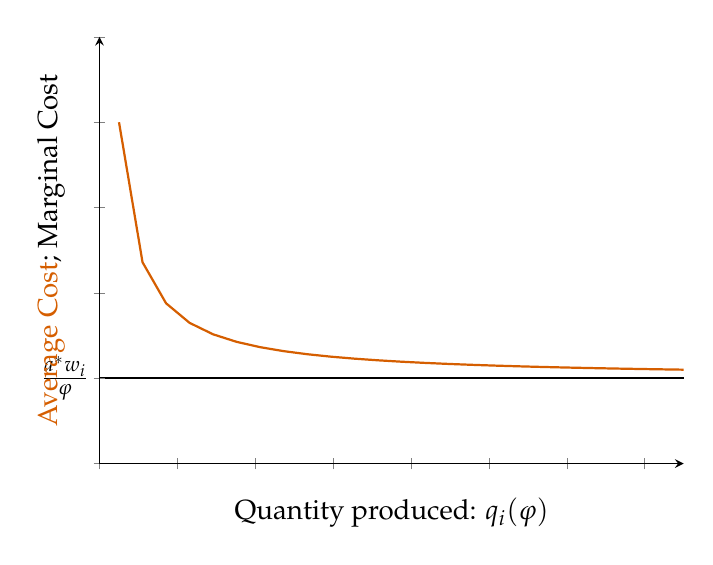
\begin{tikzpicture}

        \pgfmathsetmacro{\fbar}{1.5}
        \pgfmathsetmacro{\a}{1}
        \pgfmathsetmacro{\w}{1}
        
        \centering
        \begin{axis}[
            ylabel={\textcolor{red}{Average Cost}; Marginal Cost},
            xlabel={Quantity produced: $q_i(\varphi)$},
            ymin=0, ymax=5,
            xmin=0, xmax=15,
            yticklabel=\empty,
            xticklabel=\empty,
            axis lines=left,
            enlargelimits=false,
            clip=false,
            axis on top,
            scaled x ticks=false,
            width=9cm, height=7cm,
            title style={font=\bfseries}
        ]
        
        
          \addplot[thick,red,  domain=0.5:15]
            {\fbar/x + \a * \w};
          \addplot[thick,black,  domain=0:15]
            {\a * \w};

            \node[anchor=east] at (axis cs: 0, \a * \w) {$\frac{a^* w_i}{\varphi}$};
            
        \end{axis}
    
    \end{tikzpicture}
            \caption{Average cost as a function of output}
        \label{fig: ac}
    \end{figure}    
\end{frame}



\begin{frame}{Monopolist's maximization problem}

\begin{wideitemize}
    \item In competitive markets, producers take prices as given 
    \item Monopolists incorporate into their problem the fact that their choice of prices changes demand
    \item They take demand functions as given and pick price to maximize profits, maximizing:

    \begin{equation*}
        \max_{p(\varphi)} \pi_i(\varphi) = (p(\varphi)-MC(\varphi))q(p(\varphi)) - w_i \bar{f}
    \end{equation*}

    \blue{Solution} (using chain rule):

    \begin{equation*}
        MR(\varphi) = p(\varphi) + \frac{q(p(\varphi))}{q'(p(\varphi))} = MC(\varphi)
    \end{equation*}

\end{wideitemize}
    
\end{frame}


\section{Demand}

\begin{frame}{Demand}
    \begin{wideitemize}
        \item Consumers in country $i$ earn $w_iL_i$ and have preferences over many goods $\varphi \in \Phi_i$ 

        \begin{equation*}
            \max_{\{q_i(\
        \varphi)\}_{\
        \varphi \in \Phi_i}} Q_i \equiv \left[ \sum_{\varphi \in \Phi_i } q_i(
        \varphi)^{\tfrac{\sigma-1}{\sigma}} \right]^{\tfrac{\sigma}{\sigma-1} } \qquad s.t. \qquad  P_i Q_i =\sum_{\varphi \in \Phi_i } p_i(\varphi) q_i(\varphi) \le I_i
        \end{equation*}

        \item Is this identical as the Krugman model?

        \item<2-> Almost... Set of goods: $\varphi \in \Phi_i:=\{\varphi_{\min}, \varphi_{\min}+1, \varphi_{\min}+2, \cdots, \varphi_{\max}\}$.
        
        \item<2-> Numbering of the goods to not necessarily start at one.
        
        \item<3-> First good offered $\varphi_{\min}$, will be one of the outcomes of the equilibrium. 
        
        \item<4-> $\varphi_{\max}$ is exogenous -- the maximum possible number of goods in this economy.
        
        \item<5-> Total of $N^*=\varphi_{\max}-\varphi_{\min}+1$ goods in this economy, also endogenous. 

    \end{wideitemize}    
\end{frame}

\begin{frame}{Demand functions}
\begin{columns}
    \begin{column}{0.5\textwidth}
       After some algebra, we can solve for demand functions:            
        \begin{equation*}
            q_i(\varphi) = \underbrace{\left( \frac{p_i(\varphi)}{P_i} \right)^{-\sigma}}_{\text{relative price}} \times \underbrace{\frac{I_i}{P_i}}_{\text{real income}}
            \end{equation*}
        {\scriptsize \qquad \textcolor{gray}{(check handout for step by step derivation)}}

       \begin{wideitemize}
        \item<2-> \blue{Intuition}: demand is...
        \begin{itemize}
            \item ...decreasing in the relative price
            \item ...increasing in real aggregate income
        \end{itemize}        

        \item<3-> What about $\sigma$?
        \begin{itemize}
            \item<4-> $\sigma$ small: large change in price, small drop in demand
            \item<5-> $\sigma$ large: small change in price, large drop in demand
        \end{itemize}
        \end{wideitemize}


    \end{column}
    
    \begin{column}{0.5\textwidth}
    \onslide<6->{
    \begin{figure}[htp]
        \centering
        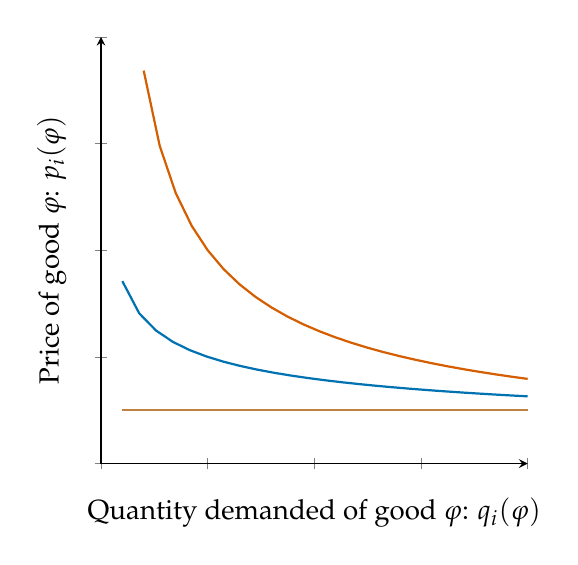
\begin{tikzpicture}
        \pgfmathsetmacro{\sigmaa}{1.5}
        \pgfmathsetmacro{\sigmab}{3}
        \pgfmathsetmacro{\sigmac}{10000000}
        \pgfmathsetmacro{\P}{0.25}
        \pgfmathsetmacro{\I}{1}
        
        \centering
        \begin{axis}[
            ylabel={Price of good $\varphi$: $p_i(\varphi)$},
            xlabel={Quantity demanded of good $\varphi$: $q_i(\varphi)$},
            ymin=0, ymax=2,
            xmin=0, xmax=2,
            yticklabel=\empty,
            xticklabel=\empty,
            axis lines=left,
            enlargelimits=false,
            clip=false,
            axis on top,
            scaled x ticks=false,
            width=7cm, height=7cm,
            title style={font=\bfseries}
        ]
        
        % PPF: Q_C = (L/a_C) - (a_R/a_C) * Q_R
    
        
          \addplot[thick,red,  domain=0.2:2]
            {\P * ((x*\P)/\I)^(-1/\sigmaa)};
          \addplot[thick,blue, domain=0.1:2]
            {\P * ((x*\P)/\I)^(-1/\sigmab)};
          \addplot[thick,brown,domain=0.1:2]
            {\P};  % σ → ∞  ⇒  horizontal line at p = P
            
        \end{axis}
    
    \end{tikzpicture}
            \caption{Demand curve with different elasticities: \textcolor{red}{$\sigma=1.5$, \textcolor{blue}{$\sigma=3$}, \textcolor{brown}{$\sigma=\infty$}}}
        \label{fig: ces-demand}
    \end{figure}
    
        }

            \end{column}
\end{columns}
\end{frame}

\section{Firm heterogeneity}

\begin{frame}{Optimal prices}

    \begin{wideitemize}
            \item From above, we know:

    \begin{equation*}
        q(p) = \left( \frac{p}{P_i} \right)^{-\sigma} \times \frac{I_i}{P_i}, \qquad q'(p) = -\sigma \times \frac{1}{p} \times \left( \frac{p}{P_i} \right)^{-\sigma} \times \frac{I_i}{P_i}  = -\sigma \times \frac{1}{p} \times q(p) 
    \end{equation*}

    \item<2-> Hence: 

    \begin{eqnarray*}
        p(\varphi) + \frac{q(p(\varphi))}{q'(p(\varphi))} &=& MC(\varphi) \\
        p(\varphi) - \frac{p(\varphi)}{\sigma} &=& MC(\varphi) \\
p(\varphi) &=& \frac{\sigma}{\sigma -1}\times MC(\varphi) = \frac{\sigma}{\sigma -1}\times \frac{a^* w_i}{\varphi}
    \end{eqnarray*}

    \item<3-> \blue{Optimal price still = mark-up $\times$ marginal cost.}

    \item<4-> But now marginal cost is firm-specific $\implies$ prices are firm-specific!

    \end{wideitemize}
\end{frame}

\begin{frame}{Diverse firms and monopolistic competition}
Firms producing different goods have different marginal costs...
\centering
    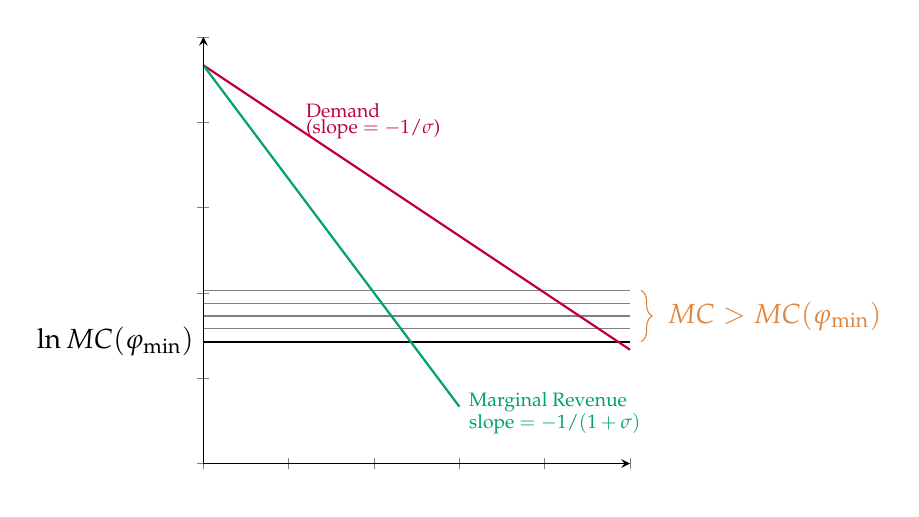
\begin{tikzpicture}
    \pgfmathsetmacro{\K}{7}
    \pgfmathsetmacro{\sigmaa}{1.5}

    \pgfmathsetmacro{\A}{7}
    \pgfmathsetmacro{\b}{0.75}
    \pgfmathsetmacro{\m}{0.35}
    \pgfmathsetmacro{\s}{2.25}
    \pgfmathsetmacro{\pmax}{\A/\b}          % choke price  (demand intercept)
    \pgfmathsetmacro{\qc}{\A - \b/\m}       % competitive quantity (P = MC)
        
    
    
    \begin{axis}[
        ymin=0, ymax=10,
        xmin=0, xmax=5,
        yticklabel=\empty,
        xticklabel=\empty,
        axis lines=left,
        enlargelimits=false,
        clip=false,
        axis on top,
        scaled x ticks=false,
        width=7cm, height=7cm,
        title style={font=\bfseries}
    ]

        
        \pgfmathsetmacro{\qs}{((\A / \b - (1/ \m  * \s) ) / ( 2/\b))}
        \pgfmathsetmacro{\ps}{ (\A / \b) - 1/\b * \qs }
        % revenue
        
        \addplot[gray, domain=0:5] {1/\m +.3};
        \addplot[gray, domain=0:5] {1/\m +.6};
        \addplot[gray, domain=0:5] {1/\m +.9};
        \addplot[gray, domain=0:5] {1/\m +1.2};

        \draw[decorate,decoration={brace,amplitude=4pt},xshift=4pt,red!75]
            (axis cs:5,1/\m +1.2) -- (axis cs:5,1/\m)
            node[midway,right=6pt]{$MC > MC(\varphi_{\min})$};

        
        
        \pgfmathsetmacro{\q}{((\A / \b - 1/ \m ) / ( 2/\b))}
        \pgfmathsetmacro{\p}{ (\A / \b) - 1/\b * \q }
        % revenue
        \addplot[black, thick, domain=0:5] {1/\m};

            %demand, rev
        \addplot[purple, thick, domain=0:5] {(\A / \b) - 1/\b * x};
        \addplot[green, thick, domain=0:3] {(\A / \b) - 2/\b * x};
            

        %\pgfmathsetmacro{\f}{\p * \q - \q / \m}
        %\addplot[blue, thick, domain=1:5] {1/\m + \f / x};

        %\addplot[gray, dashed] coordinates {(\q,1/\m + \f / \q) (0,1/\m + \f / \q)};
        %\addplot[only marks, mark=*, color=black, mark size=2pt] coordinates {(\q,1/\m + \f / \q)};


        %\node[anchor=south west] at (axis cs: 5,{1/\m+.43}) {\textcolor{blue}{Average Cost}};
        \node[anchor=south west] at (axis cs: \qs,\ps) {\scriptsize \textcolor{purple}{Demand}};
        \node[anchor=south west] at (axis cs: \qs,\ps-.5) {\scriptsize \textcolor{purple}{(slope $= - 1/\sigma$)}};
        \node[anchor=west] at (axis cs: 3,{1/(2*\m)}) {\textcolor{green}{\scriptsize Marginal Revenue}};
        \node[anchor=west] at (axis cs: 3,{1/(2*\m)-.5}) {\textcolor{green}{\scriptsize slope $= - 1/(1+\sigma)$}};

        \node[anchor=east] at (axis cs: 0,1/ \m) {$\ln  MC(\varphi_{\min})$};

    \end{axis}


    \end{tikzpicture}

 \end{frame}
 
\begin{frame}{Diverse firms and monopolistic competition}
... this is a result of the production tech for good $\varphi$...
\centering
    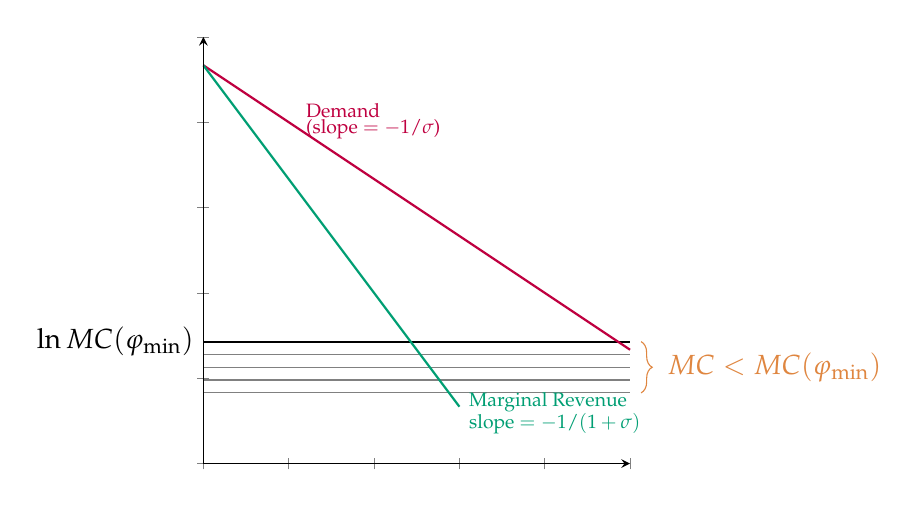
\begin{tikzpicture}
    \pgfmathsetmacro{\K}{7}
    \pgfmathsetmacro{\sigmaa}{1.5}

    \pgfmathsetmacro{\A}{7}
    \pgfmathsetmacro{\b}{0.75}
    \pgfmathsetmacro{\m}{0.35}
    \pgfmathsetmacro{\s}{2.25}
    \pgfmathsetmacro{\pmax}{\A/\b}          % choke price  (demand intercept)
    \pgfmathsetmacro{\qc}{\A - \b/\m}       % competitive quantity (P = MC)
        
    
    
    \begin{axis}[
        ymin=0, ymax=10,
        xmin=0, xmax=5,
        yticklabel=\empty,
        xticklabel=\empty,
        axis lines=left,
        enlargelimits=false,
        clip=false,
        axis on top,
        scaled x ticks=false,
        width=7cm, height=7cm,
        title style={font=\bfseries}
    ]

        
        \pgfmathsetmacro{\qs}{((\A / \b - (1/ \m  * \s) ) / ( 2/\b))}
        \pgfmathsetmacro{\ps}{ (\A / \b) - 1/\b * \qs }
        % revenue
        
        \addplot[gray, domain=0:5] {1/\m -.3};
        \addplot[gray, domain=0:5] {1/\m -.6};
        \addplot[gray, domain=0:5] {1/\m -.9};
        \addplot[gray, domain=0:5] {1/\m -1.2};

        \draw[decorate,decoration={brace,amplitude=4pt},xshift=4pt,red!75]
            (axis cs:5,1/\m) -- (axis cs:5,1/\m -1.2)
            node[midway,right=6pt]{$MC < MC(\varphi_{\min})$};

        
        
        \pgfmathsetmacro{\q}{((\A / \b - 1/ \m ) / ( 2/\b))}
        \pgfmathsetmacro{\p}{ (\A / \b) - 1/\b * \q }
        % revenue
        \addplot[black, thick, domain=0:5] {1/\m};

            %demand, rev
        \addplot[purple, thick, domain=0:5] {(\A / \b) - 1/\b * x};
        \addplot[green, thick, domain=0:3] {(\A / \b) - 2/\b * x};
            

        %\pgfmathsetmacro{\f}{\p * \q - \q / \m}
        %\addplot[blue, thick, domain=1:5] {1/\m + \f / x};

        %\addplot[gray, dashed] coordinates {(\q,1/\m + \f / \q) (0,1/\m + \f / \q)};
        %\addplot[only marks, mark=*, color=black, mark size=2pt] coordinates {(\q,1/\m + \f / \q)};


        %\node[anchor=south west] at (axis cs: 5,{1/\m+.43}) {\textcolor{blue}{Average Cost}};
        \node[anchor=south west] at (axis cs: \qs,\ps) {\scriptsize \textcolor{purple}{Demand}};
        \node[anchor=south west] at (axis cs: \qs,\ps-.5) {\scriptsize \textcolor{purple}{(slope $= - 1/\sigma$)}};
        \node[anchor=west] at (axis cs: 3,{1/(2*\m)}) {\textcolor{green}{\scriptsize Marginal Revenue}};
        \node[anchor=west] at (axis cs: 3,{1/(2*\m)-.5}) {\textcolor{green}{\scriptsize slope $= - 1/(1+\sigma)$}};

        \node[anchor=east] at (axis cs: 0,1/ \m) {$\ln  MC(\varphi_{\min})$};

    \end{axis}


    \end{tikzpicture}

 \end{frame}


\begin{frame}{Diverse firms and monopolistic competition}
Conditional on entry, each firm of a different marginal cost solves its own profit maximization problem, and chooses its own prices...
\centering
    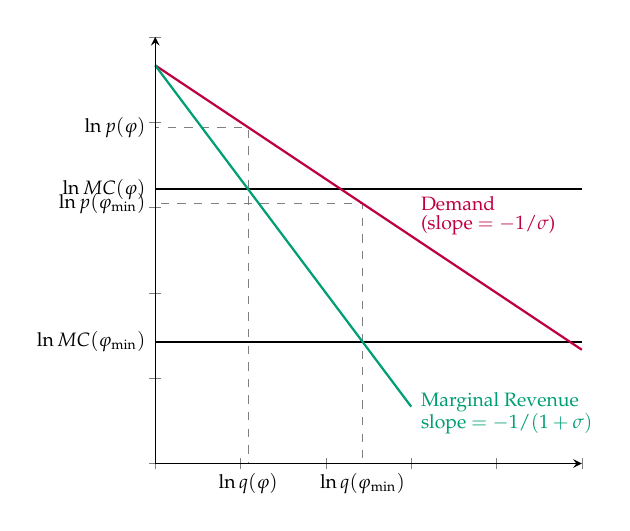
\begin{tikzpicture}
    \pgfmathsetmacro{\K}{7}
    \pgfmathsetmacro{\sigmaa}{1.5}

    \pgfmathsetmacro{\A}{7}
    \pgfmathsetmacro{\b}{0.75}
    \pgfmathsetmacro{\m}{0.35}
    \pgfmathsetmacro{\s}{2.25}
    \pgfmathsetmacro{\pmax}{\A/\b}          % choke price  (demand intercept)
    \pgfmathsetmacro{\qc}{\A - \b/\m}       % competitive quantity (P = MC)
        
    
    
    \begin{axis}[
        ymin=0, ymax=10,
        xmin=0, xmax=5,
        yticklabel=\empty,
        xticklabel=\empty,
        axis lines=left,
        enlargelimits=false,
        clip=false,
        axis on top,
        scaled x ticks=false,
        width=7cm, height=7cm,
        title style={font=\bfseries}
    ]

        
        \pgfmathsetmacro{\qs}{((\A / \b - (1/ \m  * \s) ) / ( 2/\b))}
        \pgfmathsetmacro{\ps}{ (\A / \b) - 1/\b * \qs }
        % revenue
        \addplot[gray, dashed] coordinates
            {(0,0) (0,\ps) (\qs,\ps) (\qs,0)} -- cycle;
        \addplot[black, thick, domain=0:5] {1/\m * \s};
        
        \pgfmathsetmacro{\q}{((\A / \b - 1/ \m ) / ( 2/\b))}
        \pgfmathsetmacro{\p}{ (\A / \b) - 1/\b * \q }
        % revenue
        \addplot[gray, dashed] coordinates
            {(0,0) (0,\p) (\q,\p) (\q,0)} -- cycle;
        \addplot[black, thick, domain=0:5] {1/\m};
    


            %demand, rev
        \addplot[purple, thick, domain=0:5] {(\A / \b) - 1/\b * x};
        \addplot[green, thick, domain=0:3] {(\A / \b) - 2/\b * x};
            

        %\pgfmathsetmacro{\f}{\p * \q - \q / \m}
        %\addplot[blue, thick, domain=1:5] {1/\m + \f / x};

        %\addplot[gray, dashed] coordinates {(\q,1/\m + \f / \q) (0,1/\m + \f / \q)};
        %\addplot[only marks, mark=*, color=black, mark size=2pt] coordinates {(\q,1/\m + \f / \q)};


        %\node[anchor=south west] at (axis cs: 5,{1/\m+.43}) {\textcolor{blue}{Average Cost}};
        \node[anchor=west] at (axis cs: 3,\p) {\scriptsize \textcolor{purple}{Demand}};
        \node[anchor=west] at (axis cs: 3,\p-.5) {\scriptsize \textcolor{purple}{(slope $= - 1/\sigma$)}};
        \node[anchor=west] at (axis cs: 3,{1/(2*\m)}) {\textcolor{green}{\scriptsize Marginal Revenue}};
        \node[anchor=west] at (axis cs: 3,{1/(2*\m)-.5}) {\textcolor{green}{\scriptsize slope $= - 1/(1+\sigma)$}};

        \node[anchor=east] at (axis cs: 0,1/ \m) {\scriptsize $\ln  MC(\varphi_{\min})$};
        \node[anchor=north] at (axis cs: \q,0) {\scriptsize $\ln q(\varphi_{\min})$};
        \node[anchor=east] at (axis cs: 0,\p) {\scriptsize $\ln  p(\varphi_{\min})$};

        \node[anchor=east] at (axis cs: 0,1/ \m*\s) {\scriptsize $\ln  MC(\varphi)$};
        \node[anchor=north] at (axis cs: \qs,0) {\scriptsize $\ln q(\varphi)$};
        \node[anchor=east] at (axis cs: 0,\ps) {\scriptsize $\ln  p(\varphi)$};
    \end{axis}

    \end{tikzpicture}

 \end{frame}



\begin{frame}{Firm size and productivity}

    \begin{wideitemize}
        \item When productivity and marginal costs are different across firms, they will be diverse

        \item First, more productive firms will charge lower prices: \\
        \qquad if $\varphi_{\min}>\varphi$, $p(\varphi_{\min})<p(\varphi)$

        \begin{equation*}
            p(\varphi) = \frac{\sigma}{\sigma -1}\times \frac{a^* w_i}{\varphi} \iff \frac{p(\varphi_{\min})}{p(\varphi)} = \frac{\varphi}{\varphi_{\min}} < 1
        \end{equation*}

    \end{wideitemize}
\end{frame}

\begin{frame}{Prices}

        \begin{figure}[htp]
        \centering
        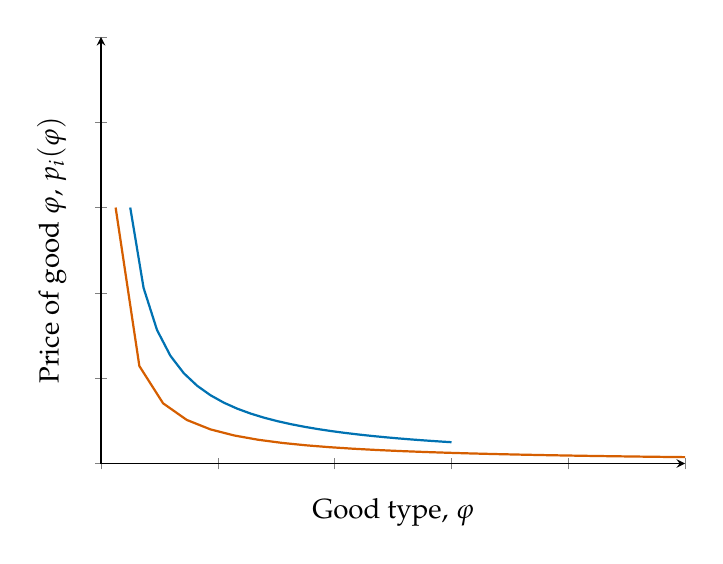
\begin{tikzpicture}

        
        \centering
        \begin{axis}[
            ylabel={Price of good $\varphi$, $p_i(\varphi)$},
            xlabel={Good type, $\varphi$},
            ymin=0, ymax=10,
            xmin=0, xmax=10,
            xticklabel=\empty,
            yticklabel=\empty,
            axis lines=left,
            enlargelimits=false,
            clip=false,
            axis on top,
            scaled x ticks=false,
            width=9cm, height=7cm,
            title style={font=\bfseries}
        ]
        
        \pgfmathsetmacro{\sigmaa}{1.5}
        \pgfmathsetmacro{\sigmab}{3}
        \pgfmathsetmacro{\a}{1}
        \pgfmathsetmacro{\w}{1}
        
          \addplot[thick,blue,  domain=0.5:6]
            {\sigmaa/(\sigmaa-1)*(\a*\w/ x ) 
            };            

          \addplot[thick,red,  domain=0.25:10]
            {\sigmab/(\sigmab-1)*(\a*\w/ x ) 
            };            
        \end{axis}
    
    \end{tikzpicture}
            \caption{Prices as a function of the good type $\varphi$ and the elasticity of substitution \textcolor{blue}{$\sigma=1.5$}, \textcolor{red}{$\sigma=3$}}
        \label{fig: ces-markup}
    \end{figure}
    
\end{frame}

\begin{frame}{Firm size and productivity}

    \begin{wideitemize}
        \item When productivity and marginal costs are different across firms, they will be diverse

        \item Second, more productive firms will earn larger revenues: \\
        \qquad if $\varphi_{\min}>\varphi$, $r_i(\varphi_{\min})>r_i(\varphi)$

        \item In particular, since $\sigma > 1$:
            \begin{eqnarray*}
    \frac{r_i(\varphi_{\min})}{r_i(\varphi)} = \left( \frac{\varphi'}{\varphi} \right)^{\sigma-1} > 1 
\end{eqnarray*}

    \qquad \textcolor{gray}{(check handout to understand how we go to this result)}


    \end{wideitemize}
\end{frame}




\begin{frame}{Revenues}
\addtocounter{framenumber}{-1}
\centering
    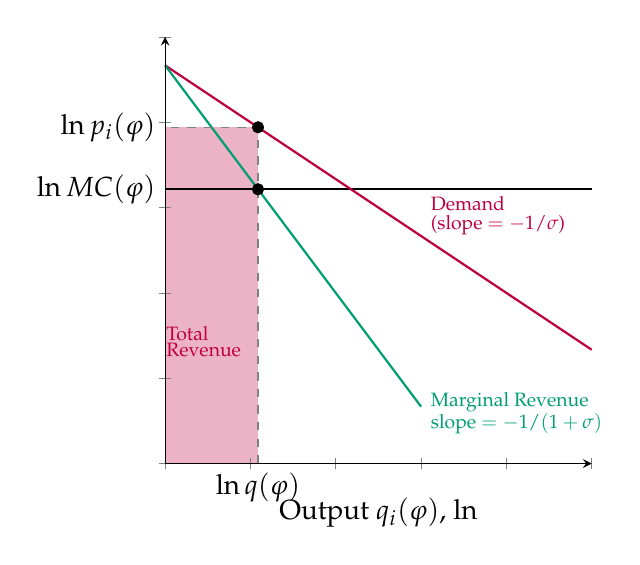
\begin{tikzpicture}
    \pgfmathsetmacro{\K}{7}
    \pgfmathsetmacro{\sigmaa}{1.5}

    \pgfmathsetmacro{\A}{7}
    \pgfmathsetmacro{\b}{0.75}
    \pgfmathsetmacro{\m}{0.35}
    \pgfmathsetmacro{\s}{2.25}
    \pgfmathsetmacro{\pmax}{\A/\b}          % choke price  (demand intercept)
    \pgfmathsetmacro{\qc}{\A - \b/\m}       % competitive quantity (P = MC)
        
    
    
    \begin{axis}[
        xlabel={Output $q_i(\varphi)$, ln},
        ymin=0, ymax=10,
        xmin=0, xmax=5,
        yticklabel=\empty,
        xticklabel=\empty,
        axis lines=left,
        enlargelimits=false,
        clip=false,
        axis on top,
        scaled x ticks=false,
        width=7cm, height=7cm,
        title style={font=\bfseries}
    ]

        \pgfmathsetmacro{\q}{((\A / \b - 1/ \m ) / ( 2/\b))}
        \pgfmathsetmacro{\p}{ (\A / \b) - 1/\b * \q }
        
        \pgfmathsetmacro{\qs}{((\A / \b - (1/ \m  * \s) ) / ( 2/\b))}
        \pgfmathsetmacro{\ps}{ (\A / \b) - 1/\b * \qs }
        % revenue
        \addplot[fill=purple!30, draw=none] coordinates
            {(0,0) (0,\ps) (\qs,\ps) (\qs,0)} -- cycle;
        \addplot[black, thick, domain=0:5] {1/\m * \s};
        


            %demand, rev
        \addplot[purple, thick, domain=0:5] {(\A / \b) - 1/\b * x};
        \addplot[green, thick, domain=0:3] {(\A / \b) - 2/\b * x};
            

        %\pgfmathsetmacro{\f}{\p * \q - \q / \m}
        %\addplot[blue, thick, domain=1:5] {1/\m + \f / x};

        
        \addplot[gray, dashed] coordinates {(\qs,0) (\qs,\ps) (0,\ps)};
        \addplot[only marks, mark=*, color=black, mark size=2pt] coordinates {(\qs,\ps)};
        \addplot[only marks, mark=*, color=black, mark size=2pt] coordinates {(\qs,1/\m * \s)};

        %\addplot[gray, dashed] coordinates {(\q,1/\m + \f / \q) (0,1/\m + \f / \q)};
        %\addplot[only marks, mark=*, color=black, mark size=2pt] coordinates {(\q,1/\m + \f / \q)};

        \node[anchor = south west] at (axis cs: -.1,{1/(\m)-.2}) {\scriptsize \textcolor{purple}{Total}};
        \node[anchor = north west] at (axis cs: -.1,{1/(\m)+.2}) {\scriptsize \textcolor{purple}{Revenue}};

        %\node[anchor=south west] at (axis cs: 5,{1/\m+.43}) {\textcolor{blue}{Average Cost}};
        \node[anchor=west] at (axis cs: 3,\p) {\scriptsize \textcolor{purple}{Demand}};
        \node[anchor=west] at (axis cs: 3,\p-.5) {\scriptsize \textcolor{purple}{(slope $= - 1/\sigma$)}};
        \node[anchor=west] at (axis cs: 3,{1/(2*\m)}) {\textcolor{green}{\scriptsize Marginal Revenue}};
        \node[anchor=west] at (axis cs: 3,{1/(2*\m)-.5}) {\textcolor{green}{\scriptsize slope $= - 1/(1+\sigma)$}};

        \node[anchor=east] at (axis cs: 0,1/ \m * \s) {$\ln  MC(\varphi)$};
        \node[anchor=east] at (axis cs: 0,\ps) {$\ln  p_i(\varphi)$};

        \node[anchor=north] at (axis cs: \qs,0) {$\ln q(\varphi)$};

    \end{axis}

    \end{tikzpicture}
 \end{frame}


\begin{frame}{Revenues}
\addtocounter{framenumber}{-1}

\centering
    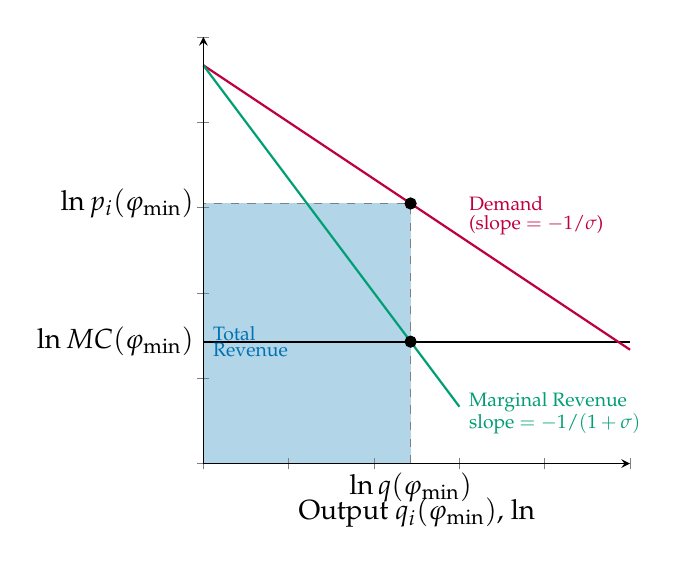
\begin{tikzpicture}
    \pgfmathsetmacro{\K}{7}
    \pgfmathsetmacro{\sigmaa}{1.5}

    \pgfmathsetmacro{\A}{7}
    \pgfmathsetmacro{\b}{0.75}
    \pgfmathsetmacro{\m}{0.35}
    \pgfmathsetmacro{\pmax}{\A/\b}          % choke price  (demand intercept)
    \pgfmathsetmacro{\qc}{\A - \b/\m}       % competitive quantity (P = MC)
        
    
    
    \begin{axis}[
        xlabel={Output $q_i(\varphi_{\min})$, ln},
        ymin=0, ymax=10,
        xmin=0, xmax=5,
        yticklabel=\empty,
        xticklabel=\empty,
        axis lines=left,
        enlargelimits=false,
        clip=false,
        axis on top,
        scaled x ticks=false,
        width=7cm, height=7cm,
        title style={font=\bfseries}
    ]

        \pgfmathsetmacro{\q}{((\A / \b - 1/ \m ) / ( 2/\b))}
        \pgfmathsetmacro{\p}{ (\A / \b) - 1/\b * \q }
        % revenue
        \addplot[fill=blue!30, draw=none] coordinates
            {(0,0) (0,\p) (\q,\p) (\q,0)} -- cycle;
        
            
        \addplot[black, thick, domain=0:5] {1/\m};
        \addplot[purple, thick, domain=0:5] {(\A / \b) - 1/\b * x};
        \addplot[green, thick, domain=0:3] {(\A / \b) - 2/\b * x};
        %\pgfmathsetmacro{\f}{\p * \q - \q / \m}
        %\addplot[blue, thick, domain=1:5] {1/\m + \f / x};

        
        \addplot[gray, dashed] coordinates {(\q,0) (\q,\p) (0,\p)};
        \addplot[only marks, mark=*, color=black, mark size=2pt] coordinates {(\q,\p)};
        \addplot[only marks, mark=*, color=black, mark size=2pt] coordinates {(\q,1/\m)};

        %\addplot[gray, dashed] coordinates {(\q,1/\m + \f / \q) (0,1/\m + \f / \q)};
        %\addplot[only marks, mark=*, color=black, mark size=2pt] coordinates {(\q,1/\m + \f / \q)};

        \node[anchor = south west] at (axis cs: 0,{1/(\m)-.2}) {\scriptsize \textcolor{blue}{Total}};
        \node[anchor = north west] at (axis cs: 0,{1/(\m)+.2}) {\scriptsize \textcolor{blue}{Revenue}};

        %\node[anchor=south west] at (axis cs: 5,{1/\m+.43}) {\textcolor{blue}{Average Cost}};
        \node[anchor=west] at (axis cs: 3,\p) {\scriptsize \textcolor{purple}{Demand}};
        \node[anchor=west] at (axis cs: 3,\p-.5) {\scriptsize \textcolor{purple}{(slope $= - 1/\sigma$)}};
        \node[anchor=west] at (axis cs: 3,{1/(2*\m)}) {\textcolor{green}{\scriptsize Marginal Revenue}};
        \node[anchor=west] at (axis cs: 3,{1/(2*\m)-.5}) {\textcolor{green}{\scriptsize slope $= - 1/(1+\sigma)$}};

        \node[anchor=east] at (axis cs: 0,1/ \m) {$\ln  MC(\varphi_{\min})$};
        \node[anchor=east] at (axis cs: 0,\p) {$\ln  p_i(\varphi_{\min})$};

        \node[anchor=north] at (axis cs: \q,0) {$\ln q(\varphi_{\min})$};

    \end{axis}

    \end{tikzpicture}

 \end{frame}


\begin{frame}{Revenues}
\centering
    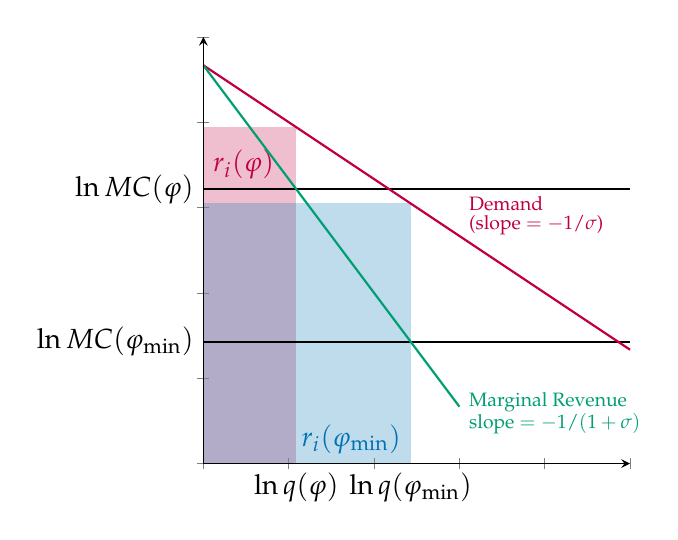
\begin{tikzpicture}
    \pgfmathsetmacro{\K}{7}
    \pgfmathsetmacro{\sigmaa}{1.5}

    \pgfmathsetmacro{\A}{7}
    \pgfmathsetmacro{\b}{0.75}
    \pgfmathsetmacro{\m}{0.35}
    \pgfmathsetmacro{\s}{2.25}
    \pgfmathsetmacro{\pmax}{\A/\b}          % choke price  (demand intercept)
    \pgfmathsetmacro{\qc}{\A - \b/\m}       % competitive quantity (P = MC)
        
    
    
    \begin{axis}[
        ymin=0, ymax=10,
        xmin=0, xmax=5,
        yticklabel=\empty,
        xticklabel=\empty,
        axis lines=left,
        enlargelimits=false,
        clip=false,
        axis on top,
        scaled x ticks=false,
        width=7cm, height=7cm,
        title style={font=\bfseries}
    ]

        
        \pgfmathsetmacro{\qs}{((\A / \b - (1/ \m  * \s) ) / ( 2/\b))}
        \pgfmathsetmacro{\ps}{ (\A / \b) - 1/\b * \qs }
        % revenue
        \addplot[fill=purple, draw=none, opacity=.25] coordinates
            {(0,0) (0,\ps) (\qs,\ps) (\qs,0)} -- cycle;
        \addplot[black, thick, domain=0:5] {1/\m * \s};
        
        \pgfmathsetmacro{\q}{((\A / \b - 1/ \m ) / ( 2/\b))}
        \pgfmathsetmacro{\p}{ (\A / \b) - 1/\b * \q }
        % revenue
        \addplot[fill=blue, draw=none, opacity=.25] coordinates
            {(0,0) (0,\p) (\q,\p) (\q,0)} -- cycle;
        \addplot[black, thick, domain=0:5] {1/\m};


        \node[anchor = south east] at (axis cs: \q,0) {\textcolor{blue}{$r_i(\varphi_{\min})$}};
    
        \node[anchor = south west] at (axis cs: 0,{\s/(\m)}) {\textcolor{purple}{$r_i(\varphi)$}};



            %demand, rev
        \addplot[purple, thick, domain=0:5] {(\A / \b) - 1/\b * x};
        \addplot[green, thick, domain=0:3] {(\A / \b) - 2/\b * x};
            

        %\pgfmathsetmacro{\f}{\p * \q - \q / \m}
        %\addplot[blue, thick, domain=1:5] {1/\m + \f / x};

        %\addplot[gray, dashed] coordinates {(\q,1/\m + \f / \q) (0,1/\m + \f / \q)};
        %\addplot[only marks, mark=*, color=black, mark size=2pt] coordinates {(\q,1/\m + \f / \q)};


        %\node[anchor=south west] at (axis cs: 5,{1/\m+.43}) {\textcolor{blue}{Average Cost}};
        \node[anchor=west] at (axis cs: 3,\p) {\scriptsize \textcolor{purple}{Demand}};
        \node[anchor=west] at (axis cs: 3,\p-.5) {\scriptsize \textcolor{purple}{(slope $= - 1/\sigma$)}};
        \node[anchor=west] at (axis cs: 3,{1/(2*\m)}) {\textcolor{green}{\scriptsize Marginal Revenue}};
        \node[anchor=west] at (axis cs: 3,{1/(2*\m)-.5}) {\textcolor{green}{\scriptsize slope $= - 1/(1+\sigma)$}};

        \node[anchor=east] at (axis cs: 0,1/ \m) {$\ln  MC(\varphi_{\min})$};
        \node[anchor=north] at (axis cs: \q,0) {$\ln q(\varphi_{\min})$};

        \node[anchor=east] at (axis cs: 0,1/ \m*\s) {$\ln  MC(\varphi)$};
        \node[anchor=north] at (axis cs: \qs,0) {$\ln q(\varphi)$};
    \end{axis}

    \end{tikzpicture}

 \end{frame}



\begin{frame}{Firm size and productivity}

    \begin{wideitemize}
        \item When productivity and marginal costs are different across firms, they will be diverse

        \item Third, more productive firms will have higher profits: \\
        \qquad if $\varphi_{\min}>\varphi$, $\pi_i(\varphi_{\min})>\pi_i(\varphi)$

        \begin{eqnarray*}
            \pi_i(\varphi) &=& \left(p(\varphi) - MC(\varphi) \right) q(\varphi) - w_i \bar{f}  \\
        \onslide<2->{
            &=& p(\varphi)q(\varphi) - \frac{\sigma-1}{\sigma} p(\varphi) q(\varphi) - w_i \bar{f}  \\
            }
        \onslide<3->{
            &=& \frac{1}{\sigma} p(\varphi)q(\varphi) - w_i \bar{f}  \\
        }
        \onslide<4->{
            &=& \frac{1}{\sigma} r_i(\varphi) - w_i \bar{f} 
        }
        \end{eqnarray*}

        \item<5-> So:        
            \begin{equation*}
                \pi_i(\varphi_{\min}) - \pi_i(\varphi) =  \frac{1}{\sigma} \left( r_i(\varphi_{\min}) - r_i(\varphi) \right) > 0
            \end{equation*}
    \end{wideitemize}
\end{frame}

\begin{frame}{Profits}
\centering
    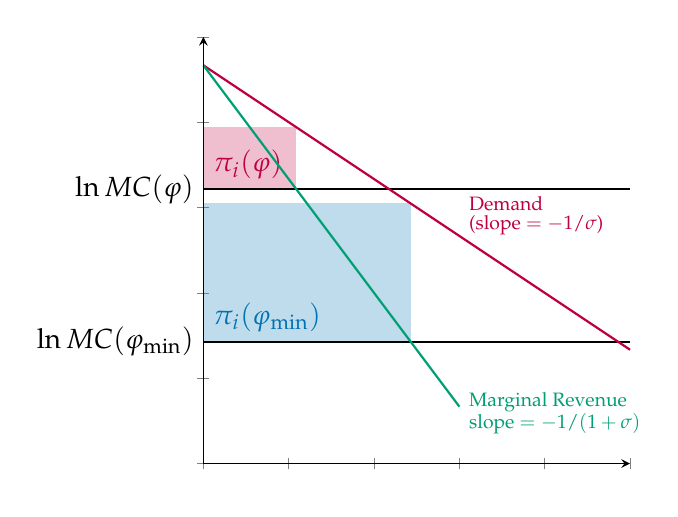
\begin{tikzpicture}
    \pgfmathsetmacro{\K}{7}
    \pgfmathsetmacro{\sigmaa}{1.5}

    \pgfmathsetmacro{\A}{7}
    \pgfmathsetmacro{\b}{0.75}
    \pgfmathsetmacro{\m}{0.35}
    \pgfmathsetmacro{\s}{2.25}
    \pgfmathsetmacro{\pmax}{\A/\b}          % choke price  (demand intercept)
    \pgfmathsetmacro{\qc}{\A - \b/\m}       % competitive quantity (P = MC)
        
    
    
    \begin{axis}[
        ymin=0, ymax=10,
        xmin=0, xmax=5,
        yticklabel=\empty,
        xticklabel=\empty,
        axis lines=left,
        enlargelimits=false,
        clip=false,
        axis on top,
        scaled x ticks=false,
        width=7cm, height=7cm,
        title style={font=\bfseries}
    ]

        
        \pgfmathsetmacro{\qs}{((\A / \b - (1/ \m  * \s) ) / ( 2/\b))}
        \pgfmathsetmacro{\ps}{ (\A / \b) - 1/\b * \qs }
        % revenue
        \addplot[fill=purple, draw=none, opacity=.25] coordinates
            {(0,1/\m*\s) (0,\ps) (\qs,\ps) (\qs,1/\m*\s)} -- cycle;
        \addplot[black, thick, domain=0:5] {1/\m * \s};
        
        \pgfmathsetmacro{\q}{((\A / \b - 1/ \m ) / ( 2/\b))}
        \pgfmathsetmacro{\p}{ (\A / \b) - 1/\b * \q }
        % revenue
        \addplot[fill=blue, draw=none, opacity=.25] coordinates
            {(0,1/\m) (0,\p) (\q,\p) (\q,1/\m)} -- cycle;
        \addplot[black, thick, domain=0:5] {1/\m};

        \node[anchor = south west] at (axis cs: 0,{1/(\m)}) {\textcolor{blue}{$\pi_i(\varphi_{\min})$}};
    
        \node[anchor = south west] at (axis cs: 0,{\s/(\m)}) {\textcolor{purple}{$\pi_i(\varphi)$}};


            %demand, rev
        \addplot[purple, thick, domain=0:5] {(\A / \b) - 1/\b * x};
        \addplot[green, thick, domain=0:3] {(\A / \b) - 2/\b * x};
            

        %\pgfmathsetmacro{\f}{\p * \q - \q / \m}
        %\addplot[blue, thick, domain=1:5] {1/\m + \f / x};

        %\addplot[gray, dashed] coordinates {(\q,1/\m + \f / \q) (0,1/\m + \f / \q)};
        %\addplot[only marks, mark=*, color=black, mark size=2pt] coordinates {(\q,1/\m + \f / \q)};


        %\node[anchor=south west] at (axis cs: 5,{1/\m+.43}) {\textcolor{blue}{Average Cost}};
        \node[anchor=west] at (axis cs: 3,\p) {\scriptsize \textcolor{purple}{Demand}};
        \node[anchor=west] at (axis cs: 3,\p-.5) {\scriptsize \textcolor{purple}{(slope $= - 1/\sigma$)}};
        \node[anchor=west] at (axis cs: 3,{1/(2*\m)}) {\textcolor{green}{\scriptsize Marginal Revenue}};
        \node[anchor=west] at (axis cs: 3,{1/(2*\m)-.5}) {\textcolor{green}{\scriptsize slope $= - 1/(1+\sigma)$}};

        \node[anchor=east] at (axis cs: 0,1/ \m) {$\ln  MC(\varphi_{\min})$};

        \node[anchor=east] at (axis cs: 0,1/ \m*\s) {$\ln  MC(\varphi)$};


    \end{axis}


    \end{tikzpicture}

 \end{frame}

\begin{frame}{Takeaways (so far)}

    \begin{wideitemize}
        \item We extended the Krugman framework to one with diverse firms
        \item Firms differ in their productivities, which means their marginal and average costs will be different
        \item With identical fixed costs, firms with different productivities optimize to different values
        \item More productive firms charge lower prices, sell higher quantities, have higher revenues and profits
    \end{wideitemize}
    
\end{frame}

\begin{frame}{Next class}
    \begin{wideitemize}
    \item This is all consistent with the broad facts we saw about exporters
    \item We will learn how to solve for the equilibrium of this model (with charts, mostly)
    \item Minimum productivity threshold $\varphi_{\min}$ will emerge in equilibrium
    \item Equilibrium number of goods available $N^*$ will also emerge in equilibrium
    \item We will also see what happens when countries open up to trade
    \end{wideitemize}
\end{frame}
%----------------------------------------------------------------------%
%----------------------------------------------------------------------%


\end{document}
